\subsection{Reminder System}
A nice feature provided by the \emph{Travlendar+} System is that it is possible to access the System either on traditional computer (through a web browser) or on a mobile phone (through the mobile application). 

In both cases, the user may want to receive a notification that suggest him to start his travel, in order to reach the location of the next task. Moreover, it may happen that the user wants to take a vehicle-shared based service, but in the very moment he starts his trip, there isn't a vehicle available. To overcome these issues, the \emph{Travlendar+} System sends a reminder to the user, and if the user wants to take a vehicle-shared based service, our System, 30 minutes before the trip starts, will check if there are vehicles available, and suggest to the user to book that vehicle.

\begin{figure}[H]
\centering
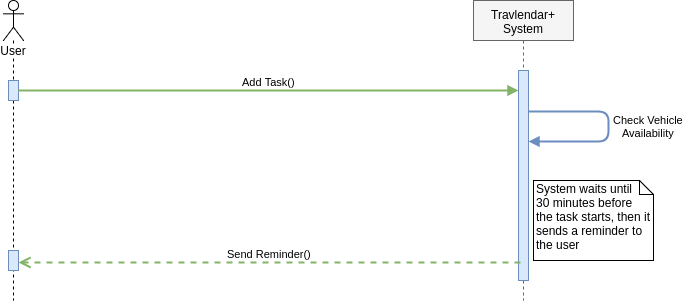
\includegraphics[scale=0.5]{Pictures/SequenceDiagram/reminder.png}
\caption{UML Sequence Diagram for the Reminder Notification System}
\end{figure}